\documentclass[../main.tex]{subfiles}

\begin{document}

\appendix 

\chapter{Codi} \label{apx: codi}
El codi emprat per entrenar els models meta-learner i analitzar els resultats està disponible al repositori de \href{https://github.com/jordi-lr/tfg-inferencia_causal}{GitHub (\texttt{jordi-lr/tfg-inferencia\_causal})}.

\chapter{Pantalles de l'aplicació Shiny} \label{apx: codi}
Aquestes són les imatges de les tres pantalles de l'aplicació Shiny.

\begin{figure}[htbp]
  \centering
  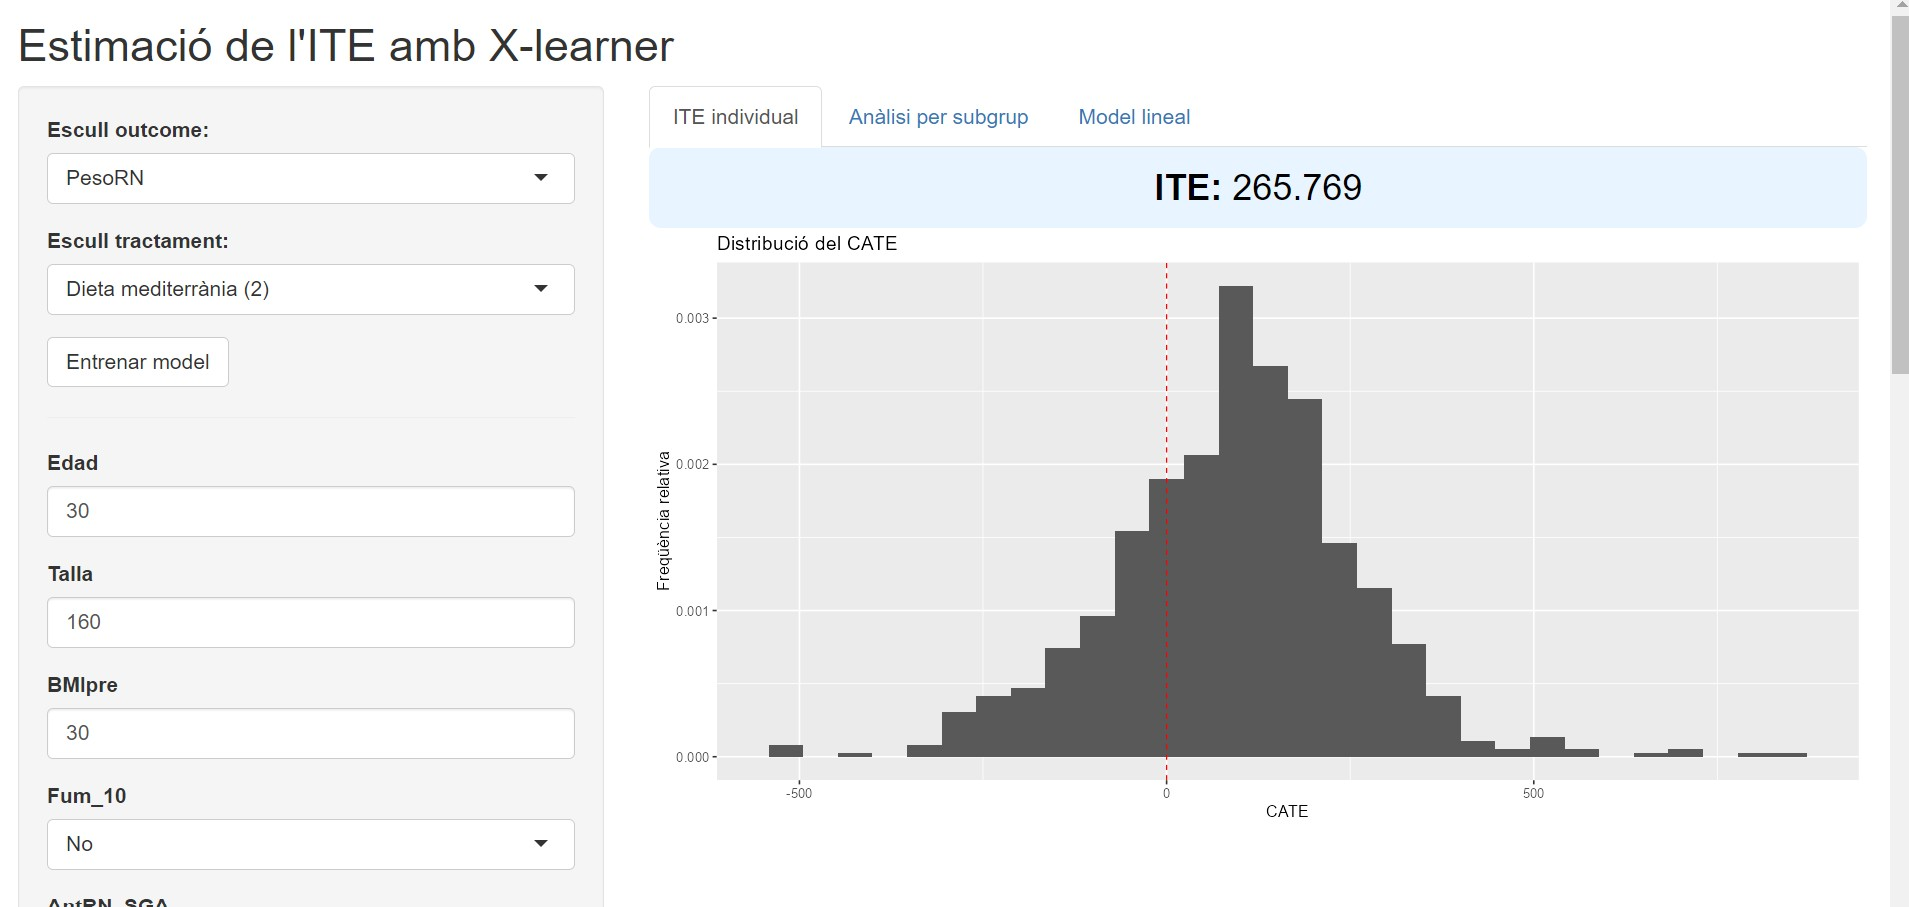
\includegraphics[width=0.8\textwidth]{imgs/pestanya1_shiny.jpg}
  \caption{Pestanya “ITE individual”: histograma amb els ITEs de la mostra i predicció de l’ITE de la nova pacient.}
  \label{fig:ite_individual}
\end{figure}

\begin{figure}[htbp]
  \centering
  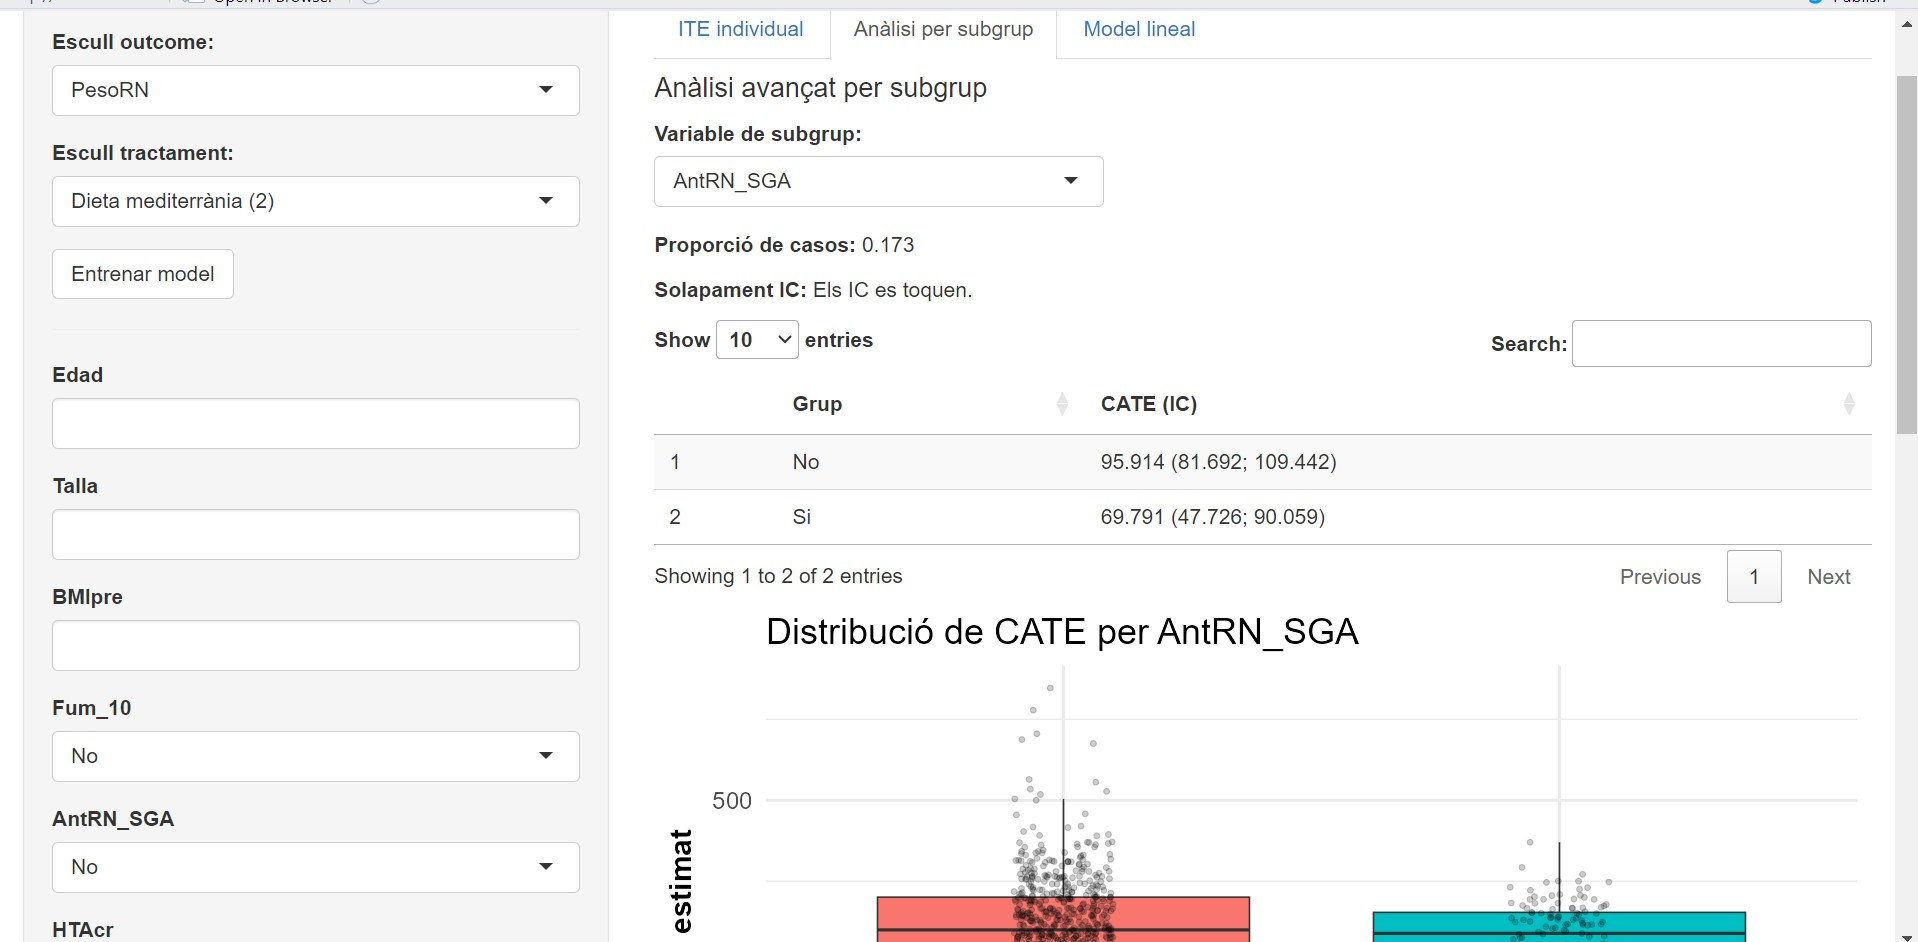
\includegraphics[width=0.8\textwidth]{imgs/pestanya2_shiny.jpg}
  \caption{Pestanya “Anàlisi per subgrup”: selecció de variable, de CATE, text de proporcions, taula d’IC i boxplot.}
  \label{fig:analisi_subgrup}
\end{figure}

\begin{figure}[htbp]
  \centering
  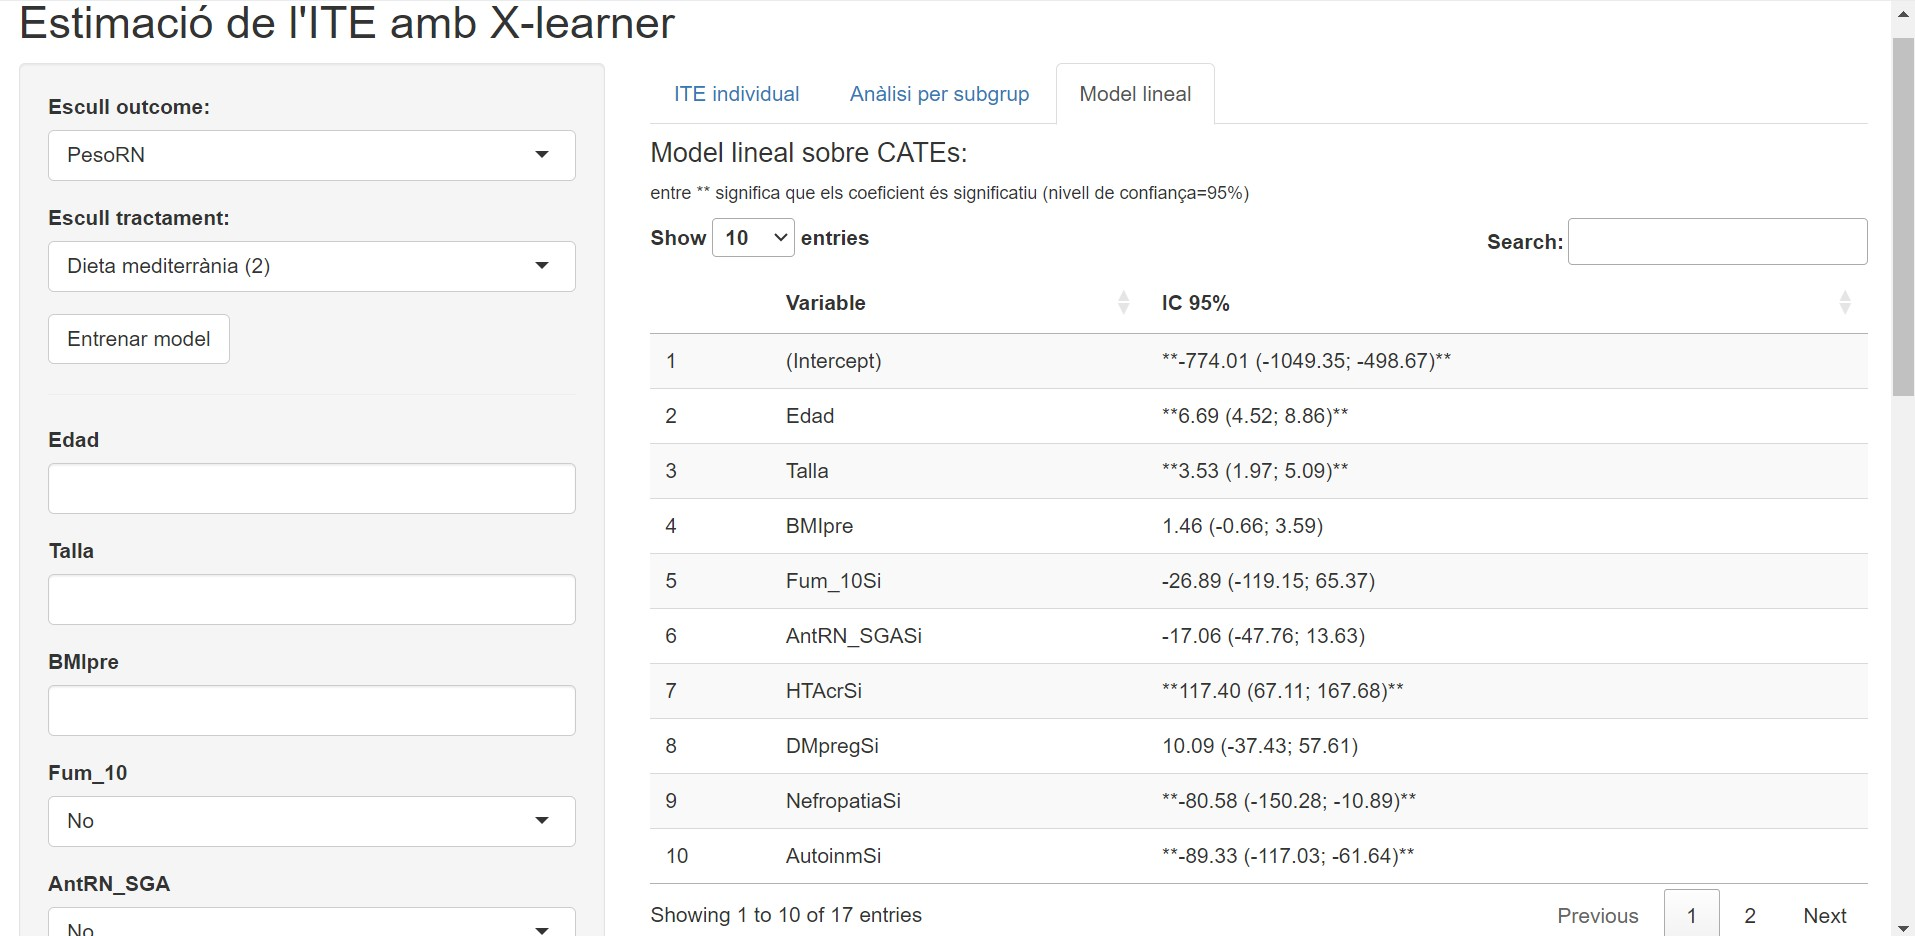
\includegraphics[width=0.8\textwidth]{imgs/pestanya3_shiny.jpg}
  \caption{Pestanya “Model lineal”: taula de coeficients amb IC al 95\%.}
  \label{fig:model_lineal}
\end{figure}


\end{document}